\chapter[Basic Statistics Examples]{Basic Statistics Examples}
\label{sec:statistics_examples}

This section introduces a few simple examples and explains a little about
computing with distributed data directly over MPI.\index{MPI} 
These implemented examples/functions are partly
selected from the Cookbook of HPSC website~\citep{hpsc2011}\index{HPSC} at
\url{http://thirteen-01.stat.iastate.edu/snoweye/hpsc/?item=cookbook}.



\section[Monte Carlo Simulation]{Monte Carlo Simulation}%\easy
\label{sec:monte_carlo}

\emph{Example:  Compute a numerical approximation for $\pi$.}

The demo command is
\begin{lstlisting}
### At the shell prompt, run the demo with 4 processors by
### (Use Rscript.exe for windows system)
mpiexec -np 4 Rscript -e "demo(monte_carlo,'pbdDEMO',ask=F,echo=F)"
\end{lstlisting}

This is a simple Monte Carlo simulation example for numerically estimating
$\pi$.
Suppose we sample $N$ uniform observations $(x_i, y_i)$ inside (or perhaps on
the border of) the unit square $[0, 1]\times [0,1]$,
where $i = 1, 2, \ldots, N$.  Then
\begin{equation}
\pi \approx 4\frac{L}{N}
\label{eqn:pi}
\end{equation}
where $0\leq L\leq N$ is the number of observations sampled satisfying
\begin{align}
x_i^2+y_i^2 \leq 1\label{math:circle}
\end{align}
The intuitive explanation for this is strategy which is sometimes given belies
a misunderstanding of infinite cardinalities, and infinite processes in
general. We are not \emph{directly} approximating an area through this
sampling scheme, because to do so with a finite-point sampling scheme would
be madness requiring a transfinite process. Indeed, let $S_N$ be the
collection of elements satisfying inequality~(\ref{math:circle}).
Then note that for each $N\in\mathbb{N}$ that the area of $S_N$ is
precisely 0. Whence,
\begin{align*}
\lim_{N\rightarrow\infty} Area(S_N) = 0
\end{align*}
This bears repeating. Finite sampling of an uncountable space requires
uncountably many such sampling operations to ``fill'' the infinite space.
For a proper treatment of set theoretic constructions, including infinite
cardinals, see \citep{kunen}.

One could argue that we are evaluating a ratio of integrals with each using
the counting measure, which satisfies technical correctness but is far from
clear. Now indeed, certain facts of area are vital here, but some care should
be taken in the discussion as to what exactly justifies our claim in
(\ref{eqn:pi}).

In reality, we are evaluating the probability that someone throwing a
0-dimensional ``dart'' at the unit square will have that ``dart'' also
land below the arc of the unit circle contained within the unit square.
Formally, let $U_1$ and $U_2$ be random uniform variables, each from the
closed unit interval $[0, 1]$.  Define the random variable
\begin{align*}
X &:= 
\begin{cases} 
1\text{, } \hspace{.4cm} U_1^2 + U_2^2 \leq 1\\ 
0\text{, \hspace{.4cm} otherwise}
\end{cases}
\end{align*}
Let $V_i = U_i^2$ for $i=1, 2$. Then the expected value
\begin{align*}
\E[X] &= \Prob( V_1 + V_2 \leq 1 )\\
     &= \int_0^1 \int_0^{1-V_1} p(V_1, V_2)dV_2 dV_1\\
     &= \int_0^1 \int_0^{1-V_1} \left( \frac{1}{2\sqrt{V_1}} \right)
        \left( \frac{1}{2\sqrt{V_2}} \right)dV_2 dV_1\\
     &= \frac{1}{2}\int_0^1 \left(\frac{1-V_1}{V_1}\right)^{1/2}dV_1\\
     &= \frac{1}{2} \left[ 
	V_1\left(\frac{1-V_1}{V_1}\right)^{1/2} 
	 - \frac{1}{2} \arctan\left(\frac{\left(\frac{1-V_1}{V_1}\right)^{1/2}
        (2V_1-1)}{2(V_1-1)}\right) 
	\right]_{V_1\rightarrow 0}^{V_1\rightarrow 1}\\
     &= \frac{1}{2}\left[ \frac{\pi}{4} +\frac{\pi}{4}  \right]
\end{align*}
and by sampling observations $X_i$ for $i=1,\dots,N$, by the Strong Law of
Large Numbers~\index{Strong Law of Large Numbers}\index{SLLN}
\begin{equation}
\bar{X}_N \stackrel{a.s.}{\longrightarrow} \frac{\pi}{4}
\hspace{.4cm} \text{ as } N\rightarrow \infty
\index{Convergence!a.s.}
\label{eqn:as_convergence}
\end{equation}
In other words,
\begin{align*}
\Prob\left(\lim_{N\rightarrow\infty} \bar{X}_N = \frac{\pi}{4}\right) = 1
\end{align*}
Whence,
\begin{align*}
\frac{L}{N} \stackrel{a.s.}{\longrightarrow} \frac{\pi}{4} \hspace{.4cm}
\text{ as } N\rightarrow \infty
\end{align*}

But because no one is going to read that, and if they do they'll just call the
author a grumpy old man,
\begin{figure}[h]
\centering
 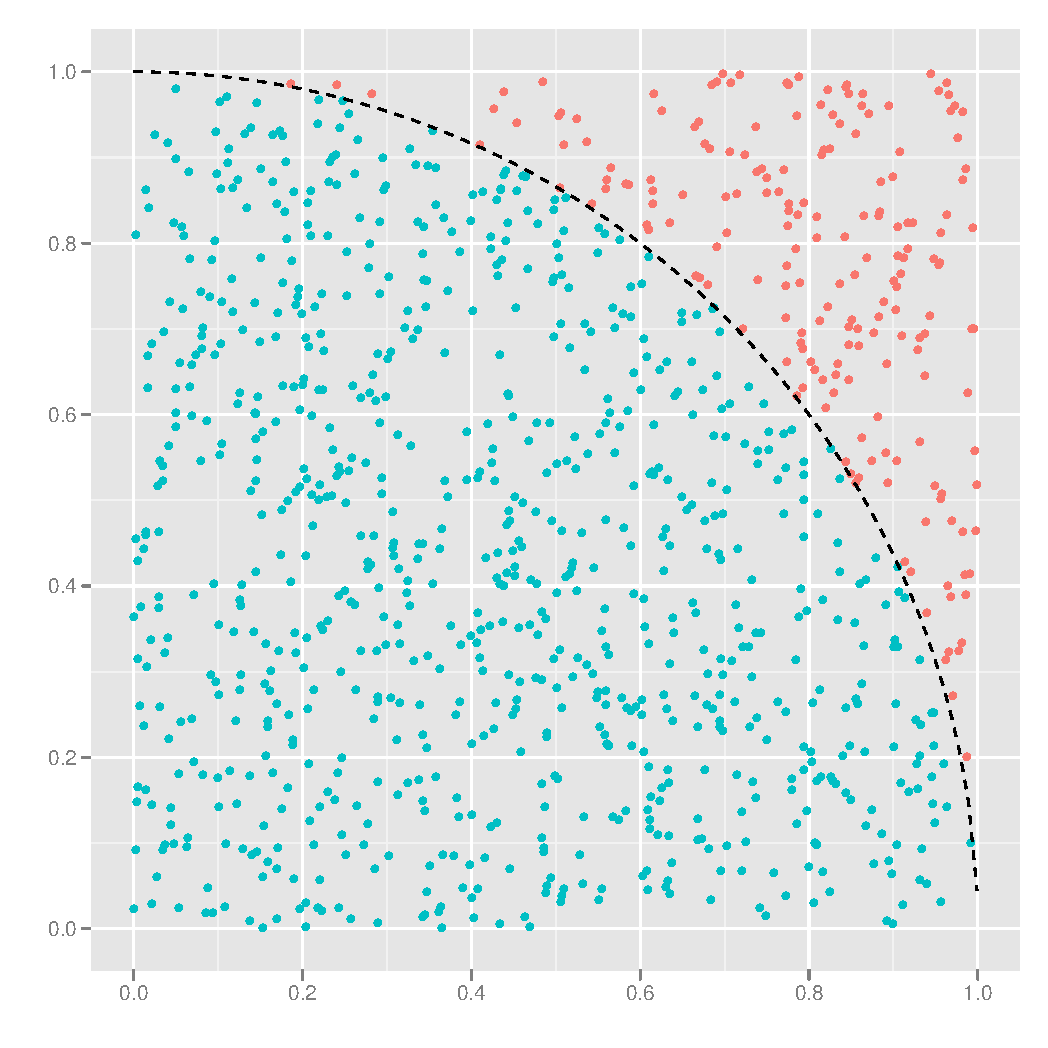
\includegraphics[height=8.5cm, width=8.5cm]{pbdDEMO-include/pics/misleading}
 \caption[Approximating $\pi$]{Approximating $\pi$ by Monte Carlo methods}\label{pic:dumb}
\end{figure}
the misleading picture you desire can be found in Figure~\ref{pic:dumb}.
And to everyone who found this looking for a homework solution, you're welcome.

The key step of the demo code is in the following block:
\begin{lstlisting}[language=rr,title=R Code]
N.spmd <- 1000
X.spmd <- matrix(runif(N.spmd * 2), ncol = 2)
r.spmd <- sum(rowSums(X.spmd^2) <= 1)
ret <- allreduce(c(N.spmd, r.spmd), op = "sum")
PI <- 4 * ret[2] / ret[1]
comm.print(PI)
\end{lstlisting}

In line 1, we specify sample size in \code{N.spmd} for each processor,
and $N=D\times\mbox{\code{N.spmd}}$ if $D$ processors are executed.
In line 2, we generate samples in \code{X.spmd} for every processor.
In line 3, we compute how many of the ``radii'' are less than or equal to $1$
for each processors.
In line 4, we call \code{allreduce()}\index{Code!\code{allreduce()}}
to obtain total numbers across all processors.
In line 5, we use the Equation~(\ref{eqn:pi}).
Since SPMD, \code{ret} is common on all processors, and so is \code{PI}.





\section[Sample Mean and Sample Variance]{Sample Mean and Sample Variance}%\easy
\label{sec:sample_stat}

\emph{Example:  Compute sample mean/variance for distributed data.}

The demo command is
\begin{lstlisting}
### At the shell prompt, run the demo with 4 processors by
### (Use Rscript.exe for windows system)
mpiexec -np 4 Rscript -e "demo(sample_stat,'pbdDEMO',ask=F,echo=F)"
\end{lstlisting}

Suppose $\bx = \{x_1, x_2, \ldots, x_N\}$
are observed samples, and $N$ is potentially very large.
We can distribute $\bx$ in 4 processors, and each processor receives a
proportional amount of data. One simple way to compute sample
mean $\bar{x}$ and
sample variance $s_x$ is based on the formulas:

\begin{align}
\bar{x} &= \frac{1}{N} \sum_{n = 1}^N x_n \notag \\[.3cm]
        &= \sum_{n = 1}^N \frac{x_n}{N} \label{math:mn}
\end{align}
and
\begin{align}
s_x     &= \frac{1}{N - 1} \sum_{n = 1}^N (x_n - \bar{x})^2 \notag \\[.3cm]
        &= \frac{1}{N - 1} \sum_{n = 1}^N x_n^2 - \frac{2\bar{x}}{N - 1}\sum_{n = 1}^N x_n +  \frac{1}{N - 1}\sum_{n = 1}^N\bar{x}^2 \notag \\[.3cm]
        &= \sum_{n = 1}^N \left(\frac{x^2_n}{N-1}\right) - \frac{N \bar{x}^2}{N-1} \label{math:sd}\\\notag
\end{align}
where expressions (\ref{math:mn}) and (\ref{math:sd}) are one-pass algorithms,
which are potentially faster than the first expressions,
especially for large $N$. However, this method of computing the variance in
one pass can suffer from round-off errors, and so in general is not
numerically stable. We provide this here for demonstration purposes only.
Additionally, only the first and second moments are implemented, while
the extension of one-pass algorithms to higher order moments is also
possible.

The demo generates random data on 4 processors, then
utilizes the \code{mpi.stat()} function:
\begin{lstlisting}[language=rr,title=R Code]
mpi.stat <- function(x.spmd){ 
  ### For mean(x).
  N <- allreduce(length(x.spmd), op = "sum")
  bar.x.spmd <- sum(x.spmd / N)
  bar.x <- allreduce(bar.x.spmd, op = "sum")

  ### For var(x).
  s.x.spmd <- sum(x.spmd^2 / (N - 1))
  s.x <- allreduce(s.x.spmd, op = "sum") - bar.x^2 * (N / (N - 1))

  list(mean = bar.x, s = s.x)
} # End of mpi.stat().
\end{lstlisting}
where \code{allreduce()}\index{Code!\code{allreduce()}}
in \pkg{pbdMPI}~\citep{Chen2012pbdMPIpackage} can
be utilized in this examples to aggregate local information across
all processors.






\section[Binning]{Binning}%\easy
\label{sec:binning}

\emph{Example:  Find binning counts for distributed data.}

The demo command is
\begin{lstlisting}
### At the shell prompt, run the demo with 4 processors by
### (Use Rscript.exe for windows system)
mpiexec -np 4 Rscript -e "demo(binning,'pbdDEMO',ask=F,echo=F)"
\end{lstlisting}

Binning is a classical problem in statistics which helps to quickly summarize
the data structure by setting some ``breaks'' between the minimum and maximum
values.
This is a particularly useful tool for constructing histograms, as well as
categorical data analysis.

The demo generates random data on 4 processors, then
utilizes the \code{mpi.bin()} function:
\begin{lstlisting}[language=rr,title=R Code]
mpi.bin <- function(x.spmd, breaks = pi / 3 * (-3:3)){
  bin.spmd <- table(cut(x.spmd, breaks = breaks))
  bin <- as.array(allreduce(bin.spmd, op = "sum"))
  dimnames(bin) <- dimnames(bin.spmd)
  class(bin) <- class(bin.spmd)
  bin
} # End of mpi.bin().
\end{lstlisting}
This simple implementation utilizes \proglang{R}'s own \code{table()}
function to obtain local counts, then calls
\code{allreduce()}\index{Code!\code{allreduce()}}
to obtain global counts on all processors.






\section[Quantile]{Quantile}%\medium
\label{sec:quantile}

\emph{Example:  Compute sample quantile order statistics for distributed data.}

The demo command is
\begin{lstlisting}
### At the shell prompt, run the demo with 4 processors by
### (Use Rscript.exe for windows system)
mpiexec -np 4 Rscript -e "demo(quantile,'pbdDEMO',ask=F,echo=F)"
\end{lstlisting}

Another fundamental tool in the statistician's toolbox is finding quantiles.
Quantiles are points taken from the cumulative distribution function.
Formally, a $q$-\emph{quantile} (or \emph{$q$-tile}) with $q~\in~[0,1]$ of
a random variable $X$ is any value $\theta_q$ such
that\footnote{This definition is due to the mathematical statistician Herman
Rubin: \url{http://mathforum.org/kb/message.jspa?messageID=406278}}
\begin{align*}
\Prob(X\leq \theta_q) &\geq q\hspace{2cm}\text{and}\\
\Prob(X\geq \theta_q) &\leq 1-q
\end{align*}
Note that by this definition, a quantile neither need exist or be unique.
Indeed, for the former, consider the
standard normal distribution\index{Distribution!normal distribution} with
$q=1$, and for the latter consider the probability 0 values of a uniform
distribution. Perhaps to narrow the scope of these problems, another
common definition is
\begin{align*}
\theta_q = \inf \{x\ |\ \Prob(X\leq x) \geq q\}
\end{align*}
In this example, we will be estimating quantiles from a sample.
Doing so requires sub-dividing the data into $q$ (almost) evenly
sized subsets, giving rise to the language $k$'th $q$-tile, for
integers $0<k<\frac{1}{q}$.

Before proceeding, we wish to make very clear the distinction between a
theoretical quantile and quantile estimation, as many web pages confuse
these two topics.  A quantile estimation from a sample requires ordering
and can take many forms; in fact, there are nine possible such forms
in \proglang{R}'s own \code{quantile()}\index{Code!\code{quantile()}}
function (see \code{help(quantile)}
in \proglang{R}). The definitions of Kendall and Cramer may be the source
of all the confusion \citep{quantilemess}. Kendall's definition, conflating
the term ``quantile'' with the act of quantile estimation, seems to have
entered most dictionaries (and Wikipedia), whereas mathematical statistics
favors the more general and simple definition of Cramer.

This example can be extended to construct Q-Q plots, compute cumulative
density function estimates and nonparametric statistics, as well as solve
maximum likelihood estimators. This is perhaps an inefficient implementation
to approximate a quantile and is not equivalent to the original
\code{quantile()} function in \proglang{R}. But in some sense, it should
work well at a large scale. The demo generates random data on 4
processors, then utilizes the \code{mpi.quantile()}:
\begin{lstlisting}[language=rr,title=R Code]
mpi.quantile <- function(x.spmd, prob = 0.5){
  if(sum(prob < 0 | prob > 1) > 0){
    stop("prob should be in (0, 1)")
  }

  N <- allreduce(length(x.spmd), op = "sum")
  x.max <- allreduce(max(x.spmd), op = "max")
  x.min <- allreduce(min(x.spmd), op = "min")

  f.quantile <- function(x, prob = 0.5){
    allreduce(sum(x.spmd <= x), op = "sum") / N - prob
  }

  uniroot(f.quantile, c(x.min, x.max), prob = prob[1])$root
} # End of mpi.quantile().
\end{lstlisting}
Here, a numerical function is solved by using
\code{uniroot()}\index{Code!\code{uniroot()}} to find out
the appropriate value where the cumulative probability is less than
or equal to the specified quantile. Specifically, it finds the zero, or root,
of the monotone \code{f.quantile()} function. This simple example shows that
with just a little effort, direct MPI methods are greatly applicable on
large scale data analysis and likelihood computing.

Note that in the way that the \code{uniroot()}
call is used above, we are legitimately operating in parallel and on
distributed data.  Other optimization functions such as
\code{optim()}\index{Code!\code{optim()}}
and \code{nlm()}\index{Code!\code{nlm()}}
can be utilized in the same way.





\section[Ordinary Least Squares]{Ordinary Least Squares}%\medium
\label{sec:ols}

\emph{Example:  Compute ordinary least square solutions for SPMD
      distributed data.}

The demo command is
\begin{lstlisting}
### At the shell prompt, run the demo with 4 processors by
### (Use Rscript.exe for windows system)
mpiexec -np 4 Rscript -e "demo(ols,'pbdDEMO',ask=F,echo=F)"
\end{lstlisting}

Ordinary least squares (OLS)\index{ordinary least squares}\index{OLS}
is perhaps \emph{the} fundamental tool of the statistician. The goal is to
find a solution $\bbeta$ such that
\begin{align}
\ltwo{ \bX\bbeta - \by }^2 \label{math:lls}
\end{align}
is minimized. In statistics, we tend to prefer to think of the problem as
being of the form
\begin{align}
\by = \bX\bbeta + \bepsilon \label{math:statslls}
\end{align}
where $\by$ is $N\times 1$ observed vector,
$\bX$ is $N\times p$ (possibly designed) matrix which is often assumed to
have full rank (more on that later), and $N >> p$,
$\bbeta$ is the unknown parameter to be estimated,
and $\bepsilon$ is errors and to be minimized in norm.

Note that above, we do indeed mean (in fact, stress) \emph{a} solution
to the linear least squares problem. For many applications a statistician
will face, expression (\ref{math:lls}) will actually have a unique
solution. But this is not always the case, and trouble often arises when
the model matrix is rank-deficient. Indeed, in this case it may occur
that there is an infinite family of solutions. So typically we go further
and demand that a solution $\bbeta$ be such that $\ltwo{\bbeta}$ is at
least as small as the corresponding norm of any other solution (although
even this may not guarantee uniqueness).

A properly thorough treatment of the problems involved here go beyond the
scope of this document, and require the reader have in-depth familiarity
with linear algebra. For our purposes, the concise explanation above will
suffice.  



In the full rank case, we can provide an analytical, ``closed-form''
solution to the problem.  In this case, the classical
% Maximum Likelihood solution
is given by:
\begin{align}
 \hat{\bbeta} = (\bX^T\bX)^{-1}\bX^T\by \label{math:ols}
\end{align}
 
This example can be also generalized to weighted least squares (WLS),
\index{weighted least squares}\index{WLS}
and linear mixed effect models.
\index{linear mixed effect models}
See \url{http://en.wikipedia.org/wiki/Least_squares} and
\url{http://en.wikipedia.org/wiki/Mixed_model} for more details.

The implementation is straight forward:
\begin{lstlisting}[language=rr,title=R Code]
if(length(y.spmd) != nrow(X.spmd)){
  stop("length(y.spmd) != nrow(X.spmd)")
}

t.X.spmd <- t(X.spmd)
A <- allreduce(t.X.spmd %*% X.spmd, op = "sum")
B <- allreduce(t.X.spmd %*% y.spmd, op = "sum")

solve(matrix(A, ncol = ncol(X.spmd))) %*% B
\end{lstlisting}

While this is a fine demonstration of the power of
``getting your hands dirty'', this approach is only efficient for
small $N$ and small $p$. This is, in large part, because the operation
is not ``fully parallel'', in that the solution is serial and replicated
on all processors. Worse, directly computing
\begin{align*}
\left(\bX^T\bX\right)^{-1}
\end{align*}
has numerical stability issues. Instead, it is generally better
(although much slower) to take an orthogonal factorization of the data matrix.
See Appendix~\ref{apx:numlinalg} for details.

Finally, all of the above assumes that the model matrix $\bX$ is full rank.
However, we have implemented an efficient method of solving linear least
squares problems in \pkg{pbdDMAT}'s
\code{lm.fit()}~\index{Code!\code{lm.fit()}}
method for distributed matrices. This method uses a fully parallel
rank-revealing QR Decomposition~\index{Decomposition!QR}
to find the least squares solution. So for larger problems, and especially
those where numerical accuracy is important or rank-degeneracy is
a possibility, it is much better to simply convert
\code{y.spmd} and \code{X.spmd}\index{Class!\code{.spmd}}
into the block-cyclic format as
in Part~\ref{part:dmat} and utilize \pkg{pbdBASE} and \pkg{pbdDMAT}
for all matrix computations.








\section{Distributed Logic}%\easy

\emph{Example:  Manage comparisons across all MPI processes.}

The demo command is
\begin{lstlisting}
### At the shell prompt, run the demo with 4 processors by
### (Use Rscript.exe for windows system)
mpiexec -np 4 Rscript -e "demo(comparators,'pbdDEMO',ask=F,echo=F)"
\end{lstlisting}

This final MPI example is not statistical in nature, but is very useful
all the same, and so we include it here. The case frequently arises where
the MPI programmer will need to do logical comparisons across all processes.
The idea is to extend the very handy \code{all()} and \code{any()}
base \proglang{R} functions to operate similarly on distributed logicals.

You could do this directly. Say you want to see if any processes
have \code{TRUE} stored in the variable \code{localLogical}.
This amounts to something on the order of:
\begin{lstlisting}[language=rr,title=R Code]
globalLogical <- as.logical(allreduce(localLogical, op='max')
\end{lstlisting}
Or you can use the function \code{comm.any()} from \pkg{pbdMPI}:
\begin{lstlisting}[language=rr,title=R Code]
globalLogical <- comm.any(localLogical)
\end{lstlisting}
which essentially does the same thing, but is more concise. Likewise,
there is a \code{comm.all()} function,\index{Code!\code{comm.all()}}
which in the equivalent ``long-form'' above would use \code{op='min'}.

The demo for these functions consists of two parts. For the first, we do a
simple demonstration of how these functions behave:
\begin{lstlisting}[language=rr,title=R Code]
rank <- comm.rank()

comm.cat("\ntest value:\n", quiet=T)
test <- (rank > 0)
comm.print(test, all.rank=T, quiet=T)

comm.cat("\ncomm.all:\n", quiet=T)
test.all <- comm.all(test)
comm.print(test.all, all.rank=T, quiet=T)

comm.cat("\ncomm.any:\n", quiet=T)
test.any <- comm.any(test)
comm.print(test.any, all.rank=T, quiet=T)
\end{lstlisting}
which should have the output:
\begin{lstlisting}[language=sh]
test value:
[1] FALSE
[1] TRUE
[1] TRUE
[1] TRUE

comm.all:
[1] FALSE
[1] FALSE
[1] FALSE
[1] FALSE

comm.any:
[1] TRUE
[1] TRUE
[1] TRUE
[1] TRUE
\end{lstlisting}

The demo also has another use case which could be very useful to a developer.
You may be interested in trying something on only one processor and then
shutting down all MPI processes if problems are encountered. To do this
in SPMD style, you can create a variable on all processes to track whether
a problem has been encountered. Then after critical code sections,
use \code{comm.any()}\index{Code!\code{comm.any()}}
to update and act appropriately.  A very simple example is provided below.

\begin{lstlisting}[language=rr,title=R Code]
need2stop <- FALSE

if (rank==0){
  need2stop <- TRUE
}

need2stop <- comm.any(need2stop)

if (need2stop)
  stop("Problem :[") 
\end{lstlisting}




\section{Exercises}
\label{sec:statistics_exercise}

\begin{enumerate}[label=\thechapter-\arabic*]
\item
What are the assumptions used in order to invoke the Strong Law of Large 
Numbers (SLLN) in statement~(\ref{eqn:as_convergence})?

\item
What is the Weak Law of Large Numbers
(WLLN)?~\index{Weak Law of Large Numbers}\index{WLLN}
Prove that the SLLN implies the WLLN. Provide a counter example that the WLLN 
does not imply the SLLN.

\item
In statement~(\ref{eqn:as_convergence}), we showed that $\bar{X}_N$ converges 
to $\frac{\pi}{4}$ almost surely,\index{Convergence!almost surely}
a very strong form of convergence.  Show that 
additionally, $\bar{X}_N$ converges to $\frac{\pi}{4}$
in probability\index{Convergence!in probability} by the 
WLLN, and that the sequence converges
in distribution.\index{Convergence!in distribution} (This can be as simple 
or as complicated as you like, depending on how many big theorems you wish to 
invoke).

\item
Let $g : [0, 1] \rightarrow  \mathbb{R}$ be a continuous function, and let 
$\bar{X}_N$ be as in statement~(\ref{eqn:as_convergence}).  Show that 
$g(\bar{X}_N)$ converges to $g\left(\frac{\pi}{4}\right)$ almost surely
{\color{blue} Hint: 
use the property of continuity with respect to limits of sequences and the 
definition of almost sure convergence.}

\item
What are assumptions for Statement~(\ref{math:statslls})?
{\color{blue} Hint: Gauss-Markov Theorem.}

\item
Prove that $\hat{\bbeta}$ of statement~(\ref{math:ols}) is an unbiased
estimator of $\bbeta$, i.e., show that $\E[ \hat{\bbeta}] = \bbeta$.
\label{ex:stat1}

\item
Prove $\bX^\top\bX$ is non-negative definite if $\bX$ has full column rank 
$p$ (and whence in this case, the inverse exists).

\item
Iteratively Reweighted Least Squares (IRLS) is an important method for finding 
solutions to generalized linear models (GLM)\footnote{See 
\url{http://en.wikipedia.org/wiki/Generalized_linear_model} for details}.  A 
common application of GLM's is logistic regression\footnote{See 
\url{http://stat.psu.edu/~jiali/course/stat597e/notes2/logit.pdf}}.

Implement a (not necessarily numerically stable) logistic regression function 
using IRLS for SPMD data.  For simplicity, you may wish to assume that the 
weighted matrix $\bX^T\textbf{W}\bX$ is full rank at each iteration.
  
\end{enumerate}

